%!TEX root = ../main.tex
\doublespacing
\chapter{Observations of Radio Scattering in the Solar Corona compared to Computational Modelling.}
\label{chap:observations_vs_theory}
As was discussed previously, the anisotropic diffusion treatment of radio wave scattering predicts certain source characteristics for a radio burst at locations from the solar disk, assuming the unscattered burst is a point source. To date, this has not been compared qualitatively to observations of Type III radio bursts. In this chapter I utilise the direct visibility fitting method described in Chapter \ref{chap:measuring_source_sizes} and apply it to hundreds of type III radio bursts. I showcase the difference between these observations and computational modelling and discuss possible causes for the discrepancy.

\section{Introduction}
\label{sec:obsvtheory_intro}
The computational modelling of radio wave scattering has seen considerable development over the 50-odd years since some of the first simulations by e.g. \cite{ Fokker1965} and \cite{Steinberg1971}.The theory for these early works followed from a generalisation of \cite{Chandrasekhar1952}, as discussed in Chapter \ref{chap:theory} and made predictions radio burst source size. \cite{Thejappa2007} further investigated the source directivity (power received from source in some solid angle compared to power from an isotropic source in the same solid angle) and time profiles of bursts using an updated correlation of isotropic density inhomogeneities. Comparisons between these models has also been a key part in the progression of the field. \cite{Stewart1972} compare the observed positions of fundamental and harmonic emission and relate it to the then contemporary scattering models \citep[e.g.][]{Fokker1965,Steinberg1971,Riddle1974}. More recently, \cite{Krupar2020} use the model of \cite{Thejappa2007} to compare the time profiles of observed radio bursts from Parker Solar probe.

The latest development in the modelling of radio wave scattering is by \cite{Kontar2019}. Rather than using the small scattering angle approximation of previous work, \cite{Kontar2019} build on the work of \cite{Arzner1999} and \cite{Bian2019} which allows for a continuous transition from weak to strong scattering. In this approach, the effect of anisotropic density inhomogeneities is treated as photon diffusion in momentum space and the Hamiltonian equations for photon position and momentum can be solved iteratively to trace a photon's path. \cite{Kontar2019} assume a spherically symmetric corona with an anisotropic distribution of electron density fluctuations (with wavenumber $\mathbf{q}$) such that $q_\parallel$ is parallel to the local radial direction. They perform Monte Carlo simulations of photons emitted from a point source at $\omega = 1.1 \omega_p(R_s)$ via fundamental plasma emission at a distance $R_s$ and an electron density from the \cite{Parker1960} density model of a spherically symmetric corona with constant temperature. The image and time profile of each burst was found by recording the arrival of each photon at some distance where scattering is considered negligible.

For a radio burst that would be observed at $\sim 35$ MHz ($f_p = \omega_p/2 \pi \sim 32$ MHz) \cite{Kontar2019} find that an anisotropy factor of $\alpha = 0.3$ is necessary to explain observations of burst decay times.  The effect of source location on the modelled image are also investigated and it is found that sources appear more elongated in the y direction close to the disk limb and almost circular at disk centre.  This effect is less evident when an anisotropy factor of $\alpha = 0.5$ is considered. Whether this relationship is observed for Type III radio bursts located at many points along the solar disk can give a certain amount of validation to recent modelling efforts and it is here where I describe the steps undertaken to do such a thing.

\section{Method}
\label{sec:obsvtheory_method}
By fitting their interferometric visibilities as described in Chapter \ref{chap:measuring_source_sizes}, the size and position of 30 Type III radio bursts over the period of 04 April 2019 to 14 April 2019 were found. The bursts were identified in LOFAR beamformed observations and their peak time determined using an automatic peak finding algorithm. Figure \ref{fig:dynamic_spectrum_070419} shows the automatically identified bursts at 30 MHz. In total, 320 bursts were identified in this way. Unfortunately, due to the strength of these bursts, the calibration of interferometric data failed for $\sim 90 \%$ of them. 30 bursts were identified manually as having successfully been calibrated and their properties fit. As well as determining the source shape and position at its peak, the area of the source over its duration was also measured. This was done by fitting a straight line to the source area over the duration of the burst, which was estimated to be 1 second before its peak and 2 seconds afterwards.

\begin{figure}
\centering
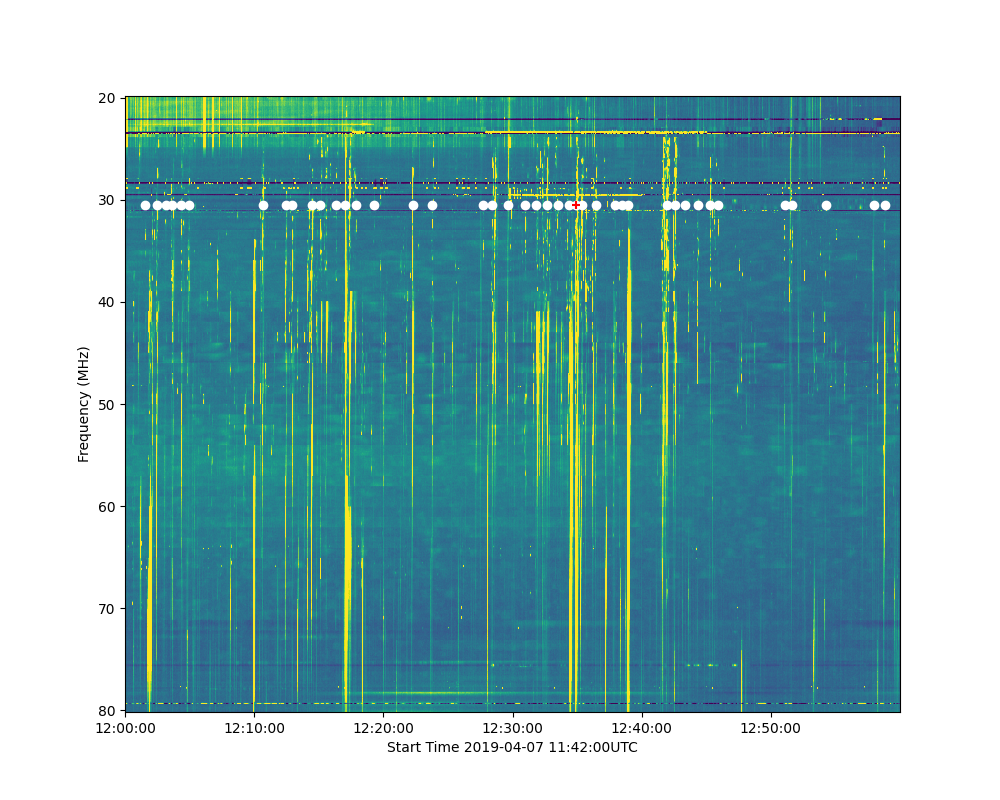
\includegraphics[width=\columnwidth]{peak_times_30MHz_2019-04-07T120000_130000.png}
\caption[Dynamic spectrum of Type III storm on 07 April 2019.]{Dynamic spectrum of Type III storm on 07 April 2019. The white dots indicate the bursts identified by an automatic peak finding algorithm, the red cross indicates the brightest burst.}
\label{fig:dynamic_spectrum_070419}
\end{figure}

\section{Results}
\label{sec:obsvtheory_results}
Each fitted type III burst is overlayed on a synoptic AIA 193\AA  map in Figure \ref{fig:synoptic_bursts}. It is clear from the figure that most burst share a similar size and ``aspect ratio", which I define as the ratio of the fwhm in the minor direction to that in the major, despite their relatively widespread origin in relation to the Sun's disk.

\begin{figure}
\centering
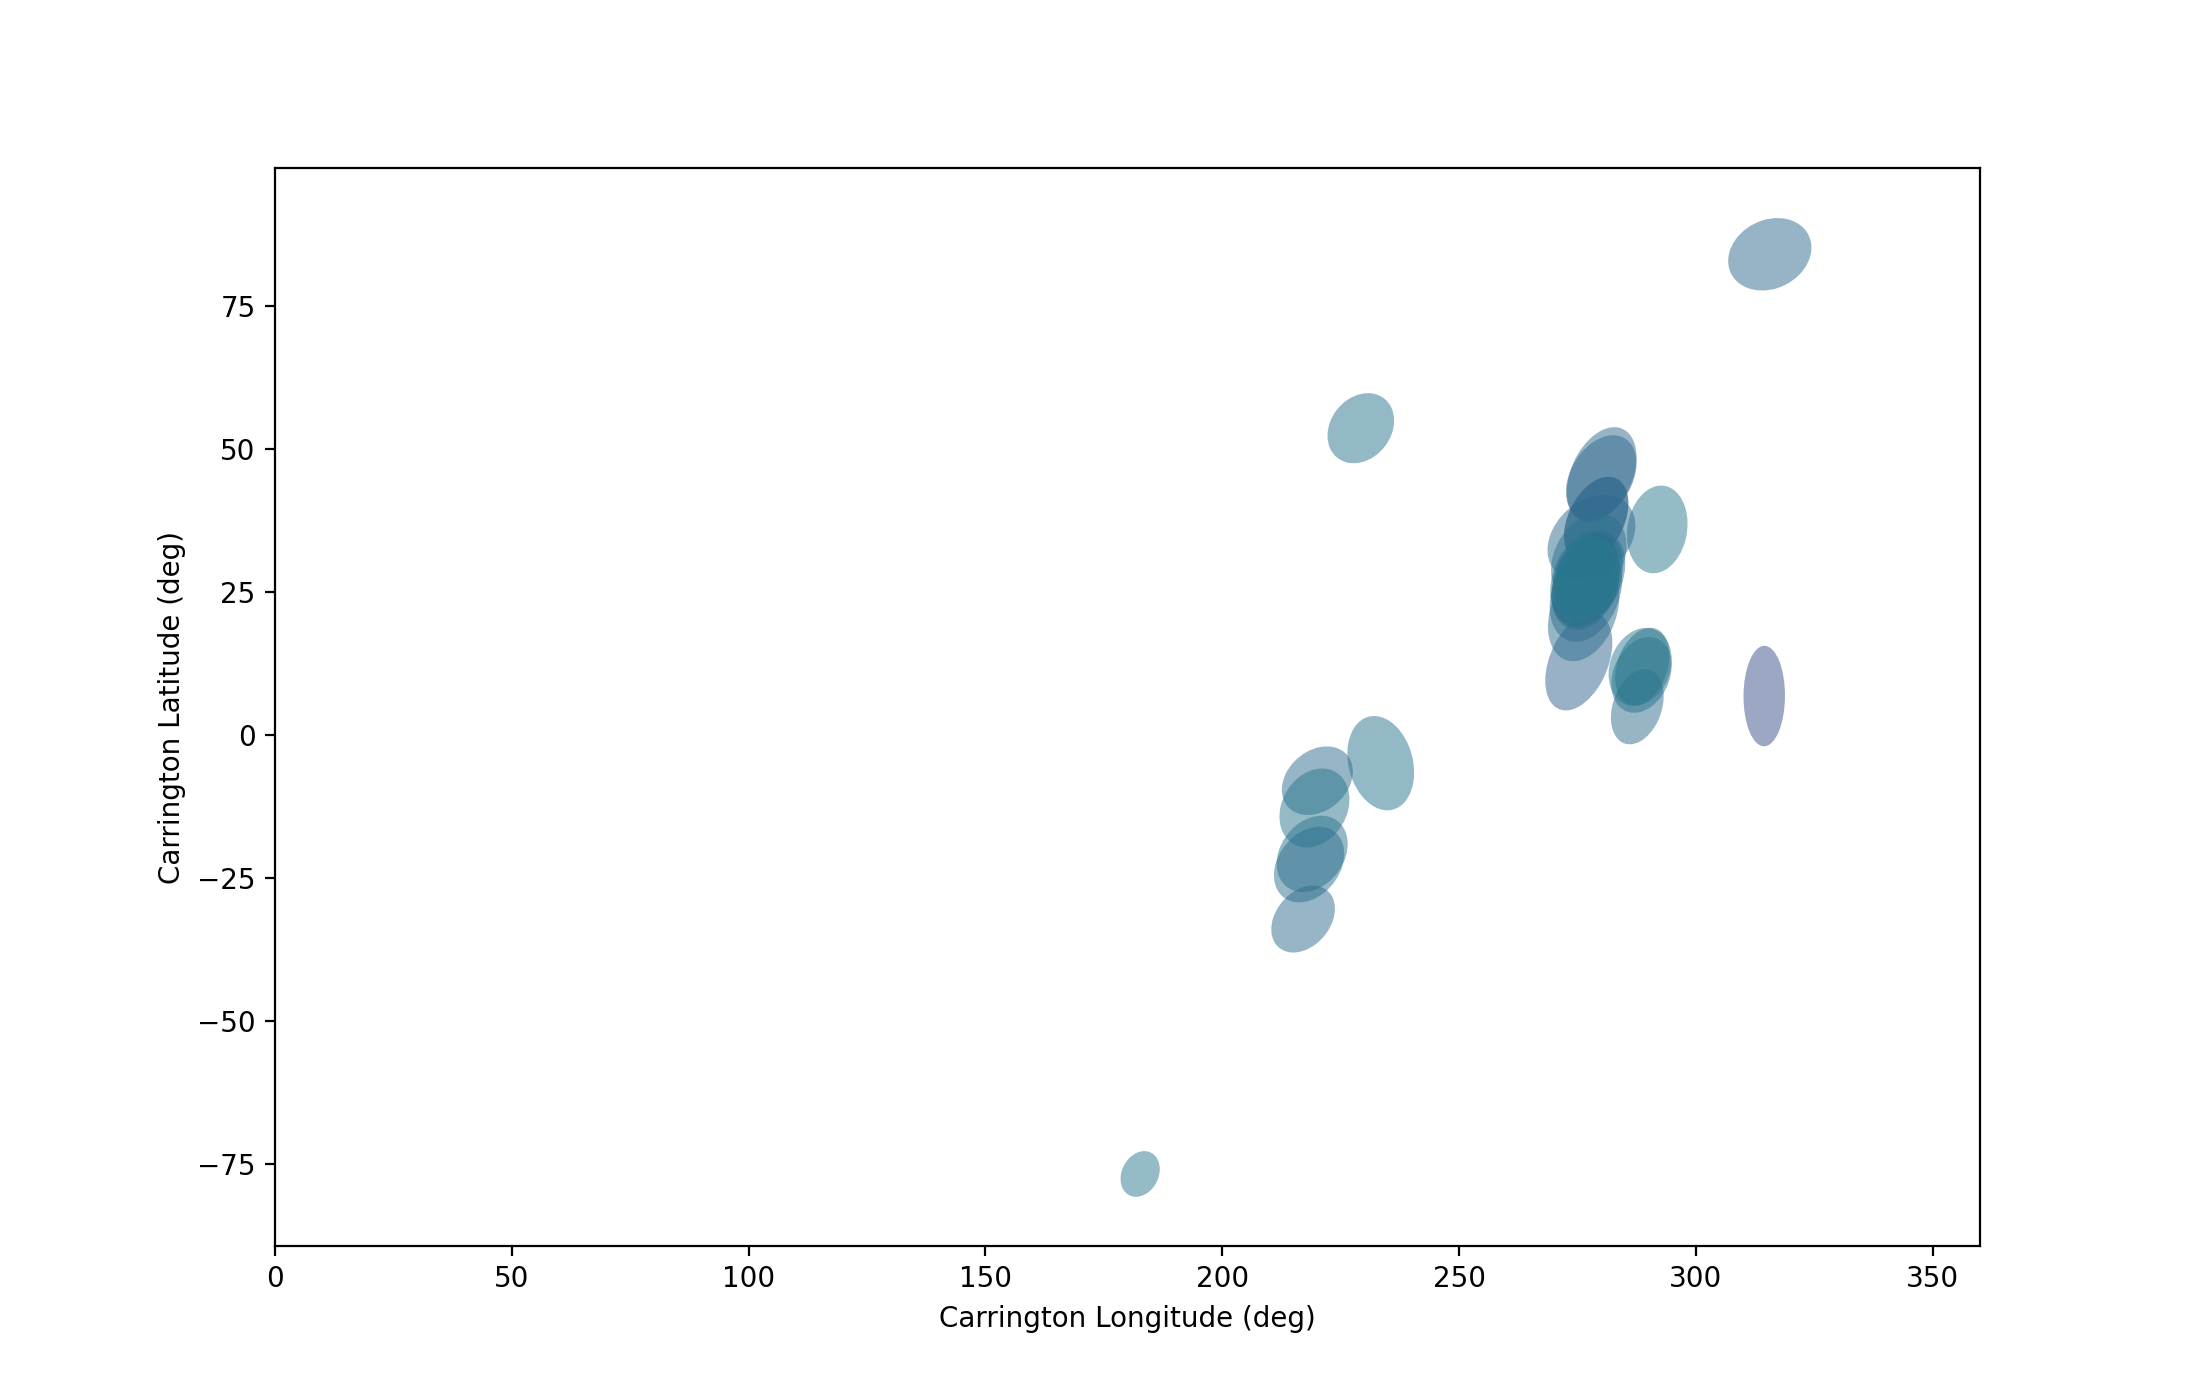
\includegraphics[width=\columnwidth]{burst_ellipses_carrington.png}
\caption[Synoptic AIA 193\AA  map overlayed with Type III radio bursts.]{A 193 \AA  AIA synoptic map where each fitted radio burst is overplotted. }
\label{fig:synoptic_bursts}
\end{figure}

\begin{landscape}
\begin{tabular}{lrrrrlrrrrrrlrrrrrr}
\toprule
{} &             I0 &    I0\_stderr &  \_\_lnsigma &  \_\_lnsigma\_stderr &                                 burst\_centre\_coord &     delta &  delta\_stderr &    redchi &     sig\_x &  sig\_x\_stderr &     sig\_y & sig\_y\_stderr &     theta &  theta\_stderr &        x0 &  x0\_stderr &        y0 &  y0\_stderr \\
\midrule
2019-04-05T12:08:08.082 &   90333.339289 &  1313.050871 &   9.276379 &          0.028606 &  <SkyCoord (Helioprojective: obstime=2019-04-05... &  0.001089 &      0.000068 &  0.999553 &  0.001082 &      0.000040 &  0.002171 &         None & -0.464067 &      0.028219 & -0.006704 &   0.000027 &  0.004480 &   0.000041 \\
2019-04-07T12:02:28.512 &   83782.443091 &   666.247493 &   8.626191 &          0.028677 &  <SkyCoord (Helioprojective: obstime=2019-04-07... &  0.000519 &      0.000036 &  0.999108 &  0.001270 &      0.000026 &  0.001789 &         None & -0.986416 &      0.035991 & -0.006885 &   0.000017 &  0.005641 &   0.000019 \\
2019-04-07T12:04:21.926 &  108123.567691 &  1092.866237 &   9.083720 &          0.028228 &  <SkyCoord (Helioprojective: obstime=2019-04-07... &  0.000399 &      0.000046 &  0.999909 &  0.001394 &      0.000035 &  0.001793 &         None & -1.163313 &      0.057581 & -0.007280 &   0.000022 &  0.005621 &   0.000025 \\
2019-04-07T12:15:07.681 &  160081.877910 &  1125.571452 &   9.048176 &          0.029151 &  <SkyCoord (Helioprojective: obstime=2019-04-07... &  0.000384 &      0.000032 &  1.000182 &  0.001542 &      0.000022 &  0.001926 &         None & -0.764279 &      0.040956 & -0.004175 &   0.000015 &  0.008723 &   0.000018 \\
2019-04-07T12:30:59.620 &  120107.741154 &   996.930357 &   9.039709 &          0.028342 &  <SkyCoord (Helioprojective: obstime=2019-04-07... &  0.000495 &      0.000038 &  0.999254 &  0.001237 &      0.000027 &  0.001731 &         None & -0.980403 &      0.039078 & -0.007610 &   0.000017 &  0.004642 &   0.000019 \\
2019-04-07T12:51:39.288 &   47916.355550 &   492.672172 &   8.272454 &          0.028768 &  <SkyCoord (Helioprojective: obstime=2019-04-07... &  0.000318 &      0.000048 &  1.000270 &  0.001501 &      0.000037 &  0.001819 &         None & -1.176700 &      0.077055 & -0.007648 &   0.000023 &  0.006023 &   0.000026 \\
2019-04-08T12:00:15.636 &  117196.685866 &  1680.726346 &   9.438227 &          0.028443 &  <SkyCoord (Helioprojective: obstime=2019-04-08... &  0.000713 &      0.000062 &  0.999378 &  0.001379 &      0.000047 &  0.002091 &         None & -1.111416 &      0.046929 & -0.002857 &   0.000033 &  0.006964 &   0.000035 \\
2019-04-08T12:00:15.636 &  117196.685866 &  1680.726346 &   9.438227 &          0.028443 &  <SkyCoord (Helioprojective: obstime=2019-04-08... &  0.000713 &      0.000062 &  0.999378 &  0.001379 &      0.000047 &  0.002091 &         None & -1.111416 &      0.046929 & -0.002857 &   0.000033 &  0.006964 &   0.000035 \\
2019-04-08T12:06:40.505 &  316272.333617 &  3295.903762 &  10.058464 &          0.028821 &  <SkyCoord (Helioprojective: obstime=2019-04-08... &  0.000685 &      0.000048 &  1.000253 &  0.001621 &      0.000036 &  0.002306 &         None & -1.145704 &      0.036186 & -0.004546 &   0.000026 &  0.006691 &   0.000027 \\
2019-04-08T12:08:36.604 &   60696.791035 &   432.567374 &   8.171062 &          0.028315 &  <SkyCoord (Helioprojective: obstime=2019-04-08... &  0.000370 &      0.000032 &  0.998452 &  0.001393 &      0.000022 &  0.001764 &         None & -0.873011 &      0.043965 & -0.004682 &   0.000015 &  0.006876 &   0.000018 \\
2019-04-08T12:22:34.290 &  171058.098235 &  1525.239020 &   9.291636 &          0.028806 &  <SkyCoord (Helioprojective: obstime=2019-04-08... &  0.000594 &      0.000041 &  0.999837 &  0.001679 &      0.000030 &  0.002273 &         None & -1.061118 &      0.035898 & -0.004228 &   0.000022 &  0.005574 &   0.000024 \\
2019-04-08T12:26:53.834 &  111428.173696 &   783.344526 &   8.664225 &          0.028705 &  <SkyCoord (Helioprojective: obstime=2019-04-08... &  0.000841 &      0.000032 &  0.999745 &  0.001469 &      0.000023 &  0.002309 &         None & -1.020291 &      0.019410 & -0.005365 &   0.000018 &  0.004483 &   0.000019 \\
2019-04-08T12:29:00.334 &   77443.586560 &   735.653212 &   8.560043 &          0.028898 &  <SkyCoord (Helioprojective: obstime=2019-04-08... &  0.000657 &      0.000044 &  1.001457 &  0.001647 &      0.000032 &  0.002304 &         None & -1.024231 &      0.034140 & -0.004362 &   0.000023 &  0.005044 &   0.000025 \\
2019-04-08T12:34:57.353 &  176944.037742 &  1895.458154 &   9.554201 &          0.028240 &  <SkyCoord (Helioprojective: obstime=2019-04-08... &  0.000629 &      0.000049 &  0.999897 &  0.001493 &      0.000037 &  0.002122 &         None & -1.252370 &      0.040744 & -0.001751 &   0.000026 &  0.005995 &   0.000026 \\
2019-04-08T12:35:35.437 &  277659.435941 &  4162.164166 &  10.297332 &          0.028221 &  <SkyCoord (Helioprojective: obstime=2019-04-08... &  0.000750 &      0.000071 &  0.998395 &  0.001531 &      0.000053 &  0.002281 &         None & -1.079573 &      0.046172 & -0.001653 &   0.000037 &  0.005860 &   0.000039 \\
2019-04-08T12:42:59.698 &  119228.985831 &  1061.991207 &   8.990948 &          0.028943 &  <SkyCoord (Helioprojective: obstime=2019-04-08... &  0.000472 &      0.000040 &  0.997425 &  0.001526 &      0.000029 &  0.001999 &         None & -1.048308 &      0.042700 & -0.005140 &   0.000020 &  0.007274 &   0.000022 \\
2019-04-08T12:47:06.994 &  155057.079088 &  1451.462677 &   9.233053 &          0.028962 &  <SkyCoord (Helioprojective: obstime=2019-04-08... &  0.000574 &      0.000043 &  0.999652 &  0.001677 &      0.000032 &  0.002251 &         None & -1.085528 &      0.039225 & -0.004328 &   0.000023 &  0.006037 &   0.000025 \\
2019-04-08T12:48:49.167 &  296662.113195 &  2600.493471 &   9.872648 &          0.028979 &  <SkyCoord (Helioprojective: obstime=2019-04-08... &  0.000514 &      0.000039 &  0.999633 &  0.001584 &      0.000029 &  0.002098 &         None & -1.074991 &      0.039390 & -0.004173 &   0.000021 &  0.005555 &   0.000023 \\
2019-04-08T12:50:26.643 &  129463.841183 &  2067.460921 &   9.571224 &          0.027900 &  <SkyCoord (Helioprojective: obstime=2019-04-08... &  0.000739 &      0.000075 &  1.001936 &  0.001682 &      0.000060 &  0.002421 &         None & -1.563606 &      0.053257 & -0.003712 &   0.000044 &  0.006819 &   0.000042 \\
2019-04-08T12:54:34.610 &  207041.119575 &  1318.801751 &   9.160834 &          0.028388 &  <SkyCoord (Helioprojective: obstime=2019-04-08... &  0.000532 &      0.000029 &  0.998699 &  0.001680 &      0.000022 &  0.002212 &         None & -1.251709 &      0.028412 & -0.004486 &   0.000016 &  0.007053 &   0.000017 \\
2019-04-08T12:59:24.856 &  177435.139321 &  1365.077605 &   9.266378 &          0.028341 &  <SkyCoord (Helioprojective: obstime=2019-04-08... &  0.000332 &      0.000036 &  1.000406 &  0.001588 &      0.000027 &  0.001920 &         None & -1.149391 &      0.053759 & -0.004768 &   0.000018 &  0.006487 &   0.000020 \\
2019-04-11T12:56:26.514 &  215905.791823 &  1521.468036 &   9.334808 &          0.028552 &  <SkyCoord (Helioprojective: obstime=2019-04-11... &  0.000476 &      0.000031 &  1.002211 &  0.001643 &      0.000019 &  0.002118 &         None & -0.008473 &      0.009564 & -0.005541 &   0.000015 &  0.002127 &   0.000021 \\
2019-04-12T12:00:18.153 &  179265.155719 &  2450.421609 &   9.824962 &          0.030087 &  <SkyCoord (Helioprojective: obstime=2019-04-12... &  0.000416 &      0.000062 &  0.996884 &  0.001409 &      0.000047 &  0.001825 &         None & -1.526534 &      0.070232 &  0.000167 &   0.000031 &  0.002676 &   0.000032 \\
2019-04-12T12:04:55.480 &  130911.177751 &  1519.411369 &   9.224042 &          0.031619 &  <SkyCoord (Helioprojective: obstime=2019-04-12... &  0.000695 &      0.000054 &  0.996640 &  0.001513 &      0.000040 &  0.002209 &         None & -1.774939 &      0.038396 &  0.001507 &   0.000030 &  0.001475 &   0.000029 \\
2019-04-12T12:14:50.568 &   43288.322505 &   538.851935 &   8.318298 &          0.028949 &  <SkyCoord (Helioprojective: obstime=2019-04-12... &  0.000499 &      0.000057 &  1.001598 &  0.001487 &      0.000044 &  0.001987 &         None & -1.452730 &      0.057504 & -0.007002 &   0.000030 &  0.000472 &   0.000030 \\
2019-04-12T12:39:31.661 &   86016.460474 &   884.112192 &   8.839200 &          0.028534 &  <SkyCoord (Helioprojective: obstime=2019-04-12... &  0.000580 &      0.000048 &  0.999925 &  0.001364 &      0.000037 &  0.001943 &         None & -1.593633 &      0.040023 & -0.004651 &   0.000024 &  0.001483 &   0.000024 \\
2019-04-12T12:49:33.963 &   74776.608394 &   854.231755 &   8.764744 &          0.028699 &  <SkyCoord (Helioprojective: obstime=2019-04-12... &  0.000401 &      0.000051 &  0.999680 &  0.001556 &      0.000040 &  0.001957 &         None & -1.391691 &      0.065276 & -0.004214 &   0.000027 &  0.000961 &   0.000028 \\
2019-04-12T12:51:54.388 &  132627.288309 &  1331.688908 &   9.221456 &          0.029037 &  <SkyCoord (Helioprojective: obstime=2019-04-12... &  0.000533 &      0.000047 &  0.999708 &  0.001450 &      0.000037 &  0.001982 &         None & -1.434764 &      0.043275 & -0.004167 &   0.000023 &  0.000202 &   0.000023 \\
2019-04-12T12:53:51.493 &  127718.173178 &   997.400885 &   9.001811 &          0.028154 &  <SkyCoord (Helioprojective: obstime=2019-04-12... &  0.000527 &      0.000035 &  1.001639 &  0.001271 &      0.000028 &  0.001798 &         None & -1.451585 &      0.033279 & -0.003884 &   0.000017 & -0.000467 &   0.000018 \\
2019-04-13T12:30:30.763 &  100613.826290 &  1207.844898 &   9.392173 &          0.028866 &  <SkyCoord (Helioprojective: obstime=2019-04-13... &  0.000218 &      0.000061 &  1.000996 &  0.000890 &      0.000049 &  0.001109 &         None & -1.321743 &      0.123145 & -0.002026 &   0.000021 & -0.003131 &   0.000024 \\
\bottomrule
\label{tab:dataset}
\end{tabular}
\caption{Table caption}
\end{landscape}

The size of each burst, here denoted by the full width half maximum in the major and minor direction, is plotted against the distance from the disk centre in the x and y direction in Figure \ref{fig:fwhm_comp}. There is no obvious trend towards bigger/smaller bursts with increasing distance from disk centre and, most strikingly, in direct contrast to the prediction by \cite{Kontar2019} there is no trend in the ``aspect ratio" of the bursts, which is expected to trend towards 1 near disk centre and $< 1$ near the limb. The mean size of the bursts $\sim 16$ arcmin and $\sim 11$ arcmin in the major and minor directions respectively. This is consistent with previous work at these frequencies \citep{Kontar2017, Murphy2021}.

\begin{figure}
\centering
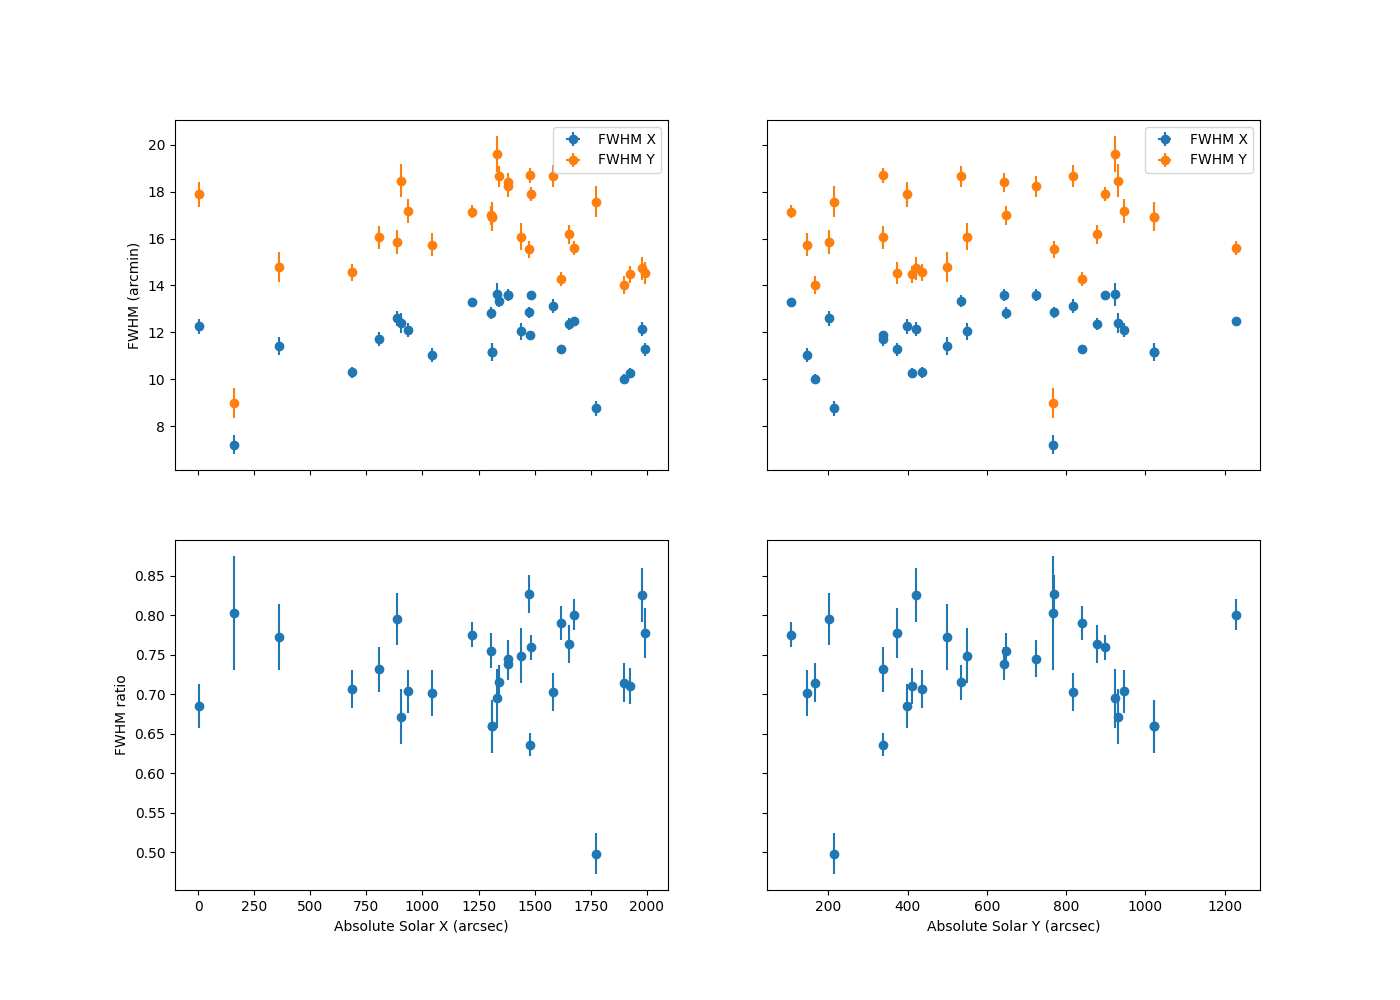
\includegraphics[width=\columnwidth]{fwhm_comparison.png}
\caption[Directly fitted Type III burst sizes as a function of position relative to disk centre.]{A comparison of the directly fitted Type III burst sizes and their location relative to the disk centre in the x and y direction. Top row, FWHM in x (blue) and y (orange) as a function of their distance from the disk centre in the x (left) and y (right) direction. Bottom row, same as above except showing the ``aspect ratio" of each burst.}
\label{fig:fwhm_comp}
\end{figure}

\section{Discussion}
\label{sec:obsvtheory_discussion}
The results given here are largely consistent with models of scattering through anisotropic density fluctuations in a spherically symmetric corona as presented by \cite{Kontar2019}. However, there is one major deviation in the results; no trend of source size vs heliocentric angle is evident in the data. The simplest, and perhaps most appropriate, answer to why this is the case is mentioned in the discussion of \cite{Kontar2019}. Since their work only analyses the path of photons from a point source, it is possible that Type III (and all other) radio bursts have an intrinsic source size. The total observed size then can be considered as the intrinsic size and the size due to scattering of a point source added in quadrature FWHM\textsubscript{total} = (FWHM\textsuperscript{2}\textsubscript{intrinsic} + FWHM\textsuperscript{2}\textsubscript{scattering})$^{1/2}$. Therefore, no trend in source sizes could suggest an intrinsic size greater than the size due to scattering. Interestingly, however, there appears to be a relationship in the orientation of the major axis of bursts being almost perpendicular to the radial line from solar centre. This suggest some form of aniostropic process... Another alternative is that the degree of aniostropy is in fact smaller than suggested by \cite{Kontar2019} and is closer to $\alpha = 0.5$, or even that it is not constant with time and or position (i.e. not axially symmetric as the MC method is based off of)
